%Title: Literature studies for I262
%Author: A. Raggio
%Year: 2020

\documentclass[10pt]{beamer}

%
%Setting file
%

\usepackage[T1]{fontenc}
\usepackage[utf8]{inputenc}

\usepackage[english]{babel}

\usepackage{graphicx}
\graphicspath{{images/}}
\usepackage{float}
\usepackage{tikz}
\usepackage{caption}
\usepackage{subcaption}

\usetheme{default}
\usefonttheme{structurebold}


% ---------------------------------
% color definitions
\usepackage{color}
% \definecolor{LISA_BLUE}{rgb}{0.25,0.33,0.66}
\definecolor{LISA_BLUE}{cmyk}{0.99,0.88,0.29,0.18}

\setbeamercolor{normal text}{fg=LISA_BLUE}
\setbeamercolor{frametitle}{fg=LISA_BLUE}

\newcommand\insertlocation{}  % Empty by default.
\newcommand\location[1]{\renewcommand\insertlocation{#1}}

\newcommand\insertperiod{}  % Empty by default.
\newcommand\period[1]{\renewcommand\insertperiod{#1}}



\setbeamertemplate{itemize items}[circle]
\setbeamercolor{title}{fg=white}



%-----------------------------------------Title page settings-----------------------------------------%
\title{\normalsize Mass 226}

\institute{}

\author{}


\date{}
\titlegraphic{% 
\vspace{0.05\textheight}
	\centering
	
\includegraphics[height=3cm]{jyu-keskitetty-kaksikielinen.eps}\\
\vspace{-0.03\textheight}
}
%-----------------------------------------Title page settings-----------------------------------------%


\setbeamertemplate{footline}
{
 \begin{beamercolorbox}{section in head/foot}
 \vskip2pt\hspace{0.095cm} Andrea Raggio \hfill Jyv\"{a}skyl\"{a} - 2021 \hspace{0.15cm}\phantom{x}\vskip2pt
 \end{beamercolorbox}%
}


\begin{document}
\frame{\titlepage}
\begin{frame}{Production rates $^{224}$Th and $^{224}$Pa}	
	\centering
	\vspace{-0.05\textheight}
	$^{224}$Th $\rightarrow$ 42.4~mbar $\rightarrow$ $(79\% \text{ main }\alpha\text{ branch})$ 33.50~mbar\\
	$^{224}$Pa $\rightarrow$ 40.5~mbar $\rightarrow$ $(70\% \text{ main }\alpha\text{ branch})$ 28.35~mbar\\
	\textcolor{red}{Expected Ratio $^{224}$Th/$^{224}$Pa} $\rightarrow$ $\sim$1.2 \textcolor{red}{Measured} $\rightarrow$ $\sim$3.7 
	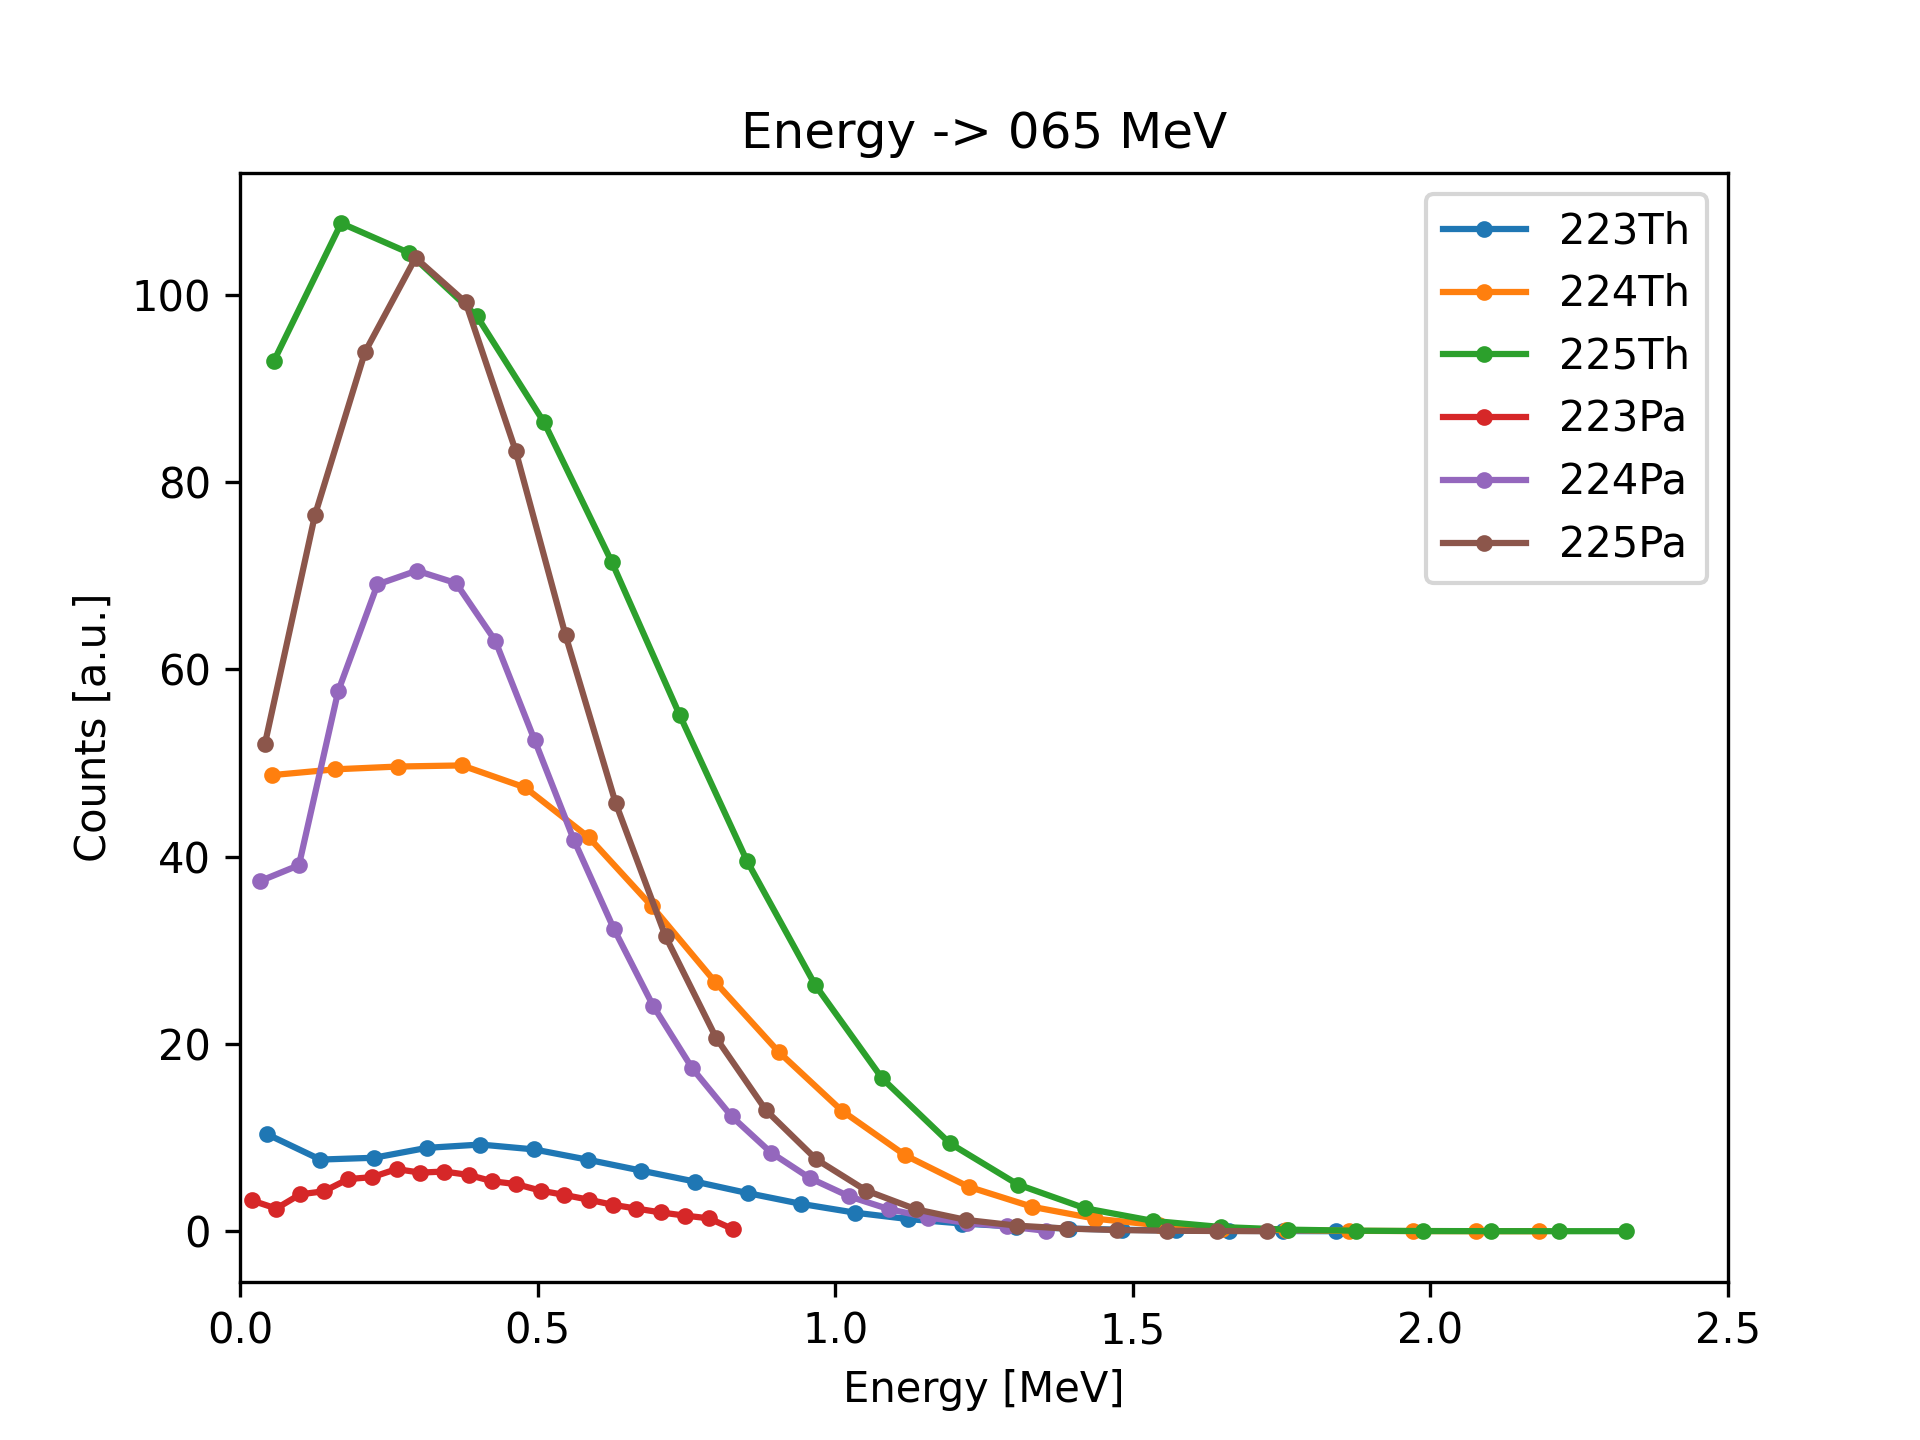
\includegraphics[width=0.7\textwidth]{Recoils.png}
\end{frame}

\begin{frame}{Mass 226}	
	\centering
	\vspace{-0.05\textheight}
	\hspace*{-0.05\textwidth}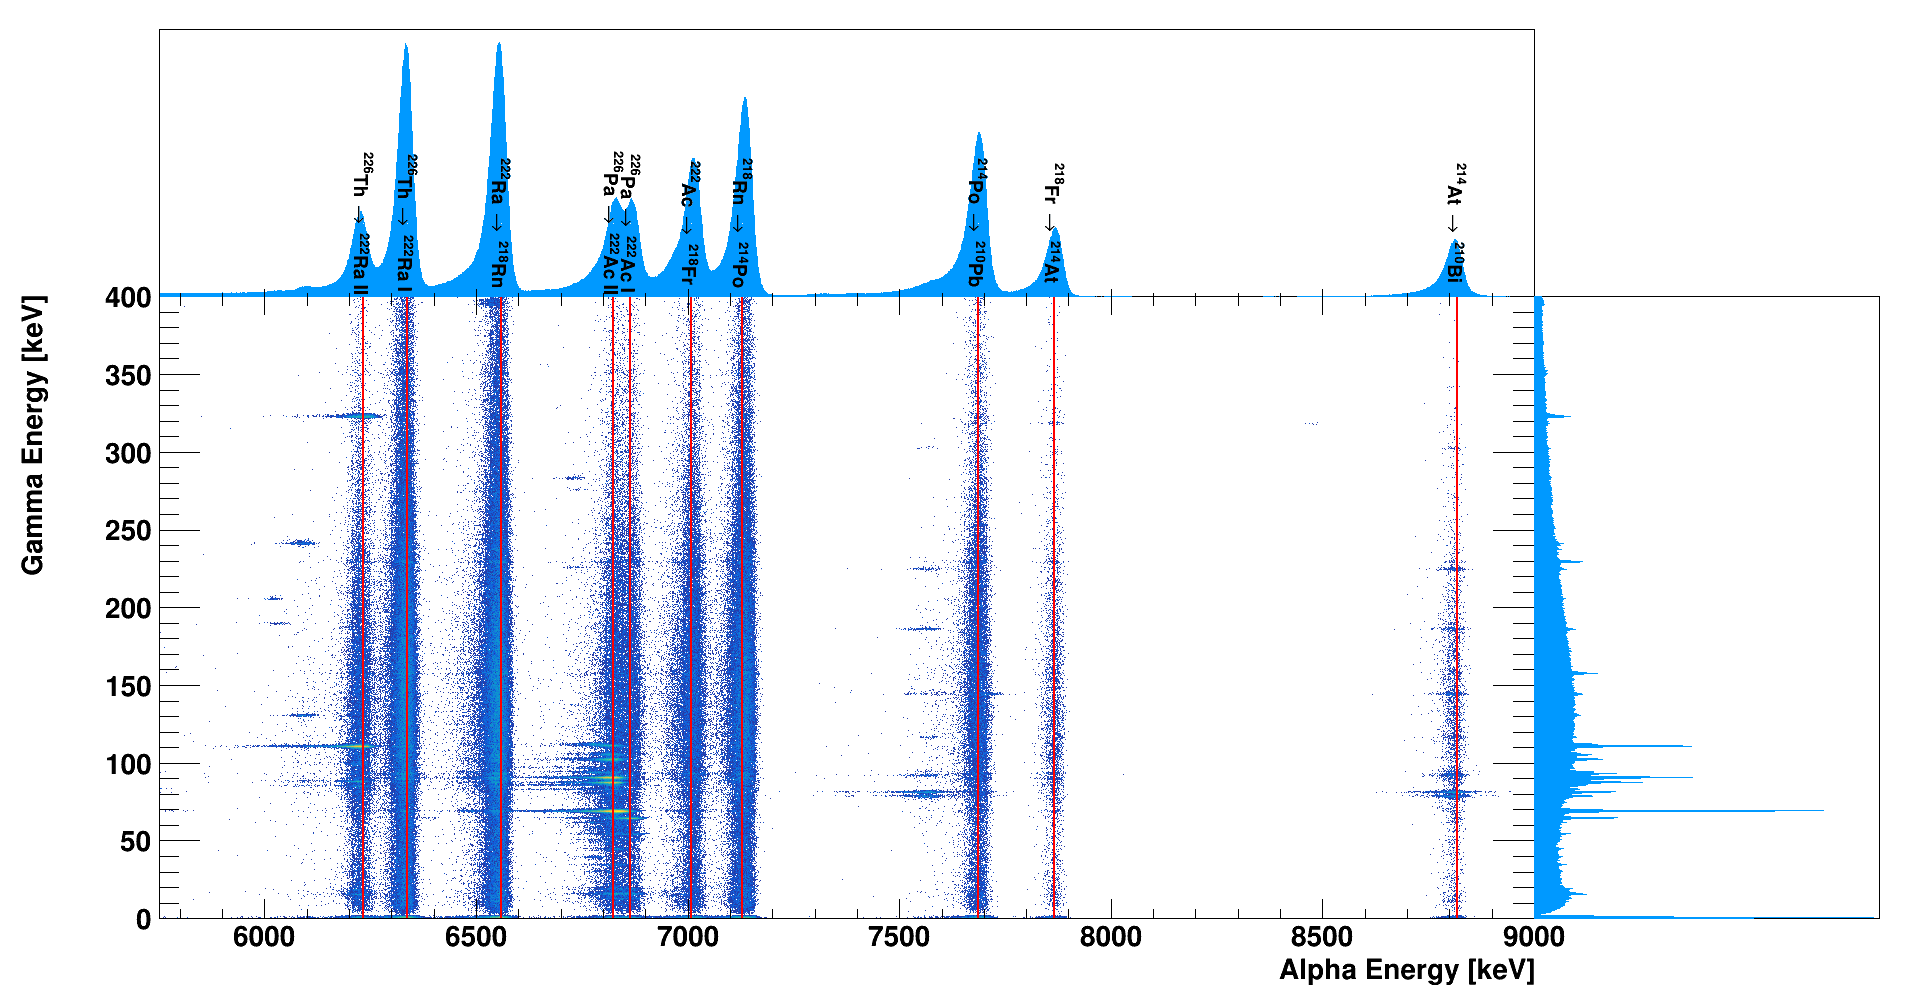
\includegraphics[width=1.1\textwidth]{AvsG_10us.png}
\end{frame}

\begin{frame}{Mass 226}	
	\begin{columns}
		\begin{column}{0.5\textwidth}
			\begin{overlayarea}{\textwidth}{0.5\textheight}
				\centering
				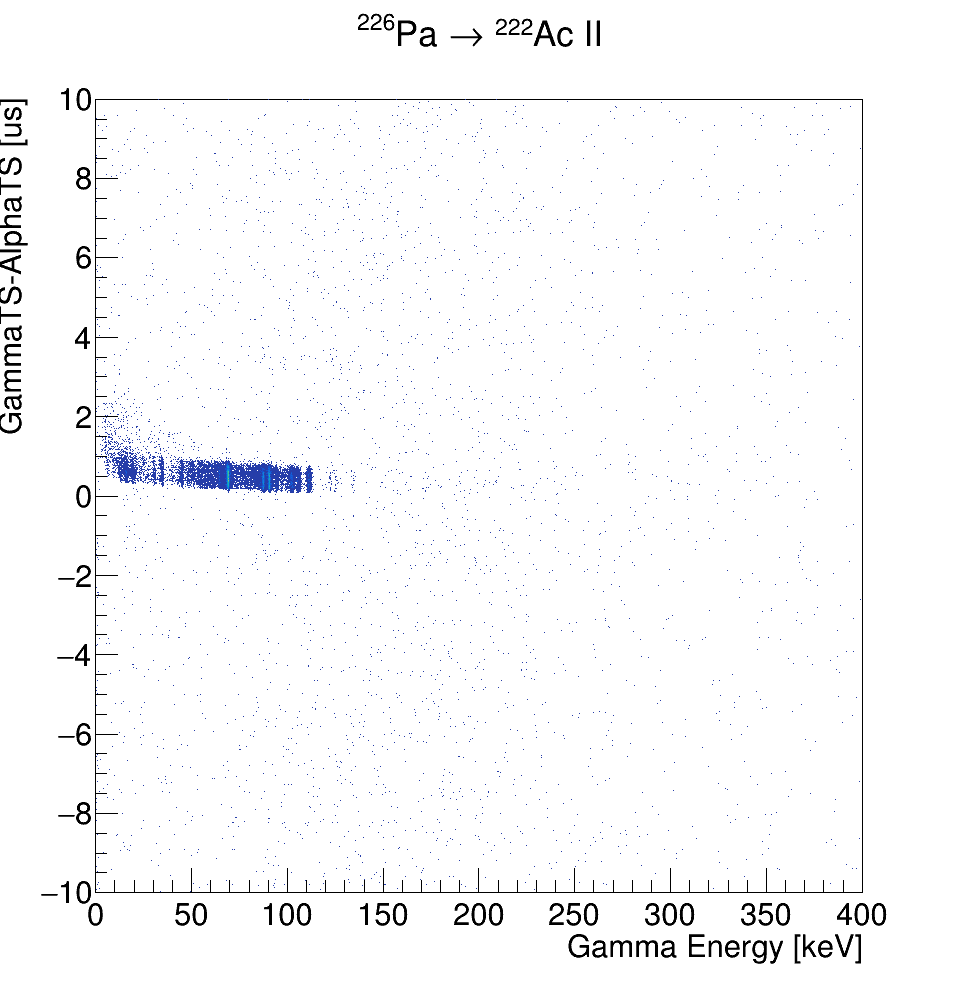
\includegraphics[width=\textwidth]{GTvsG_226Pa.png}
			\end{overlayarea}
		\end{column}
		\begin{column}{0.5\textwidth}
			\begin{overlayarea}{\textwidth}{0.5\textheight}
				\centering
				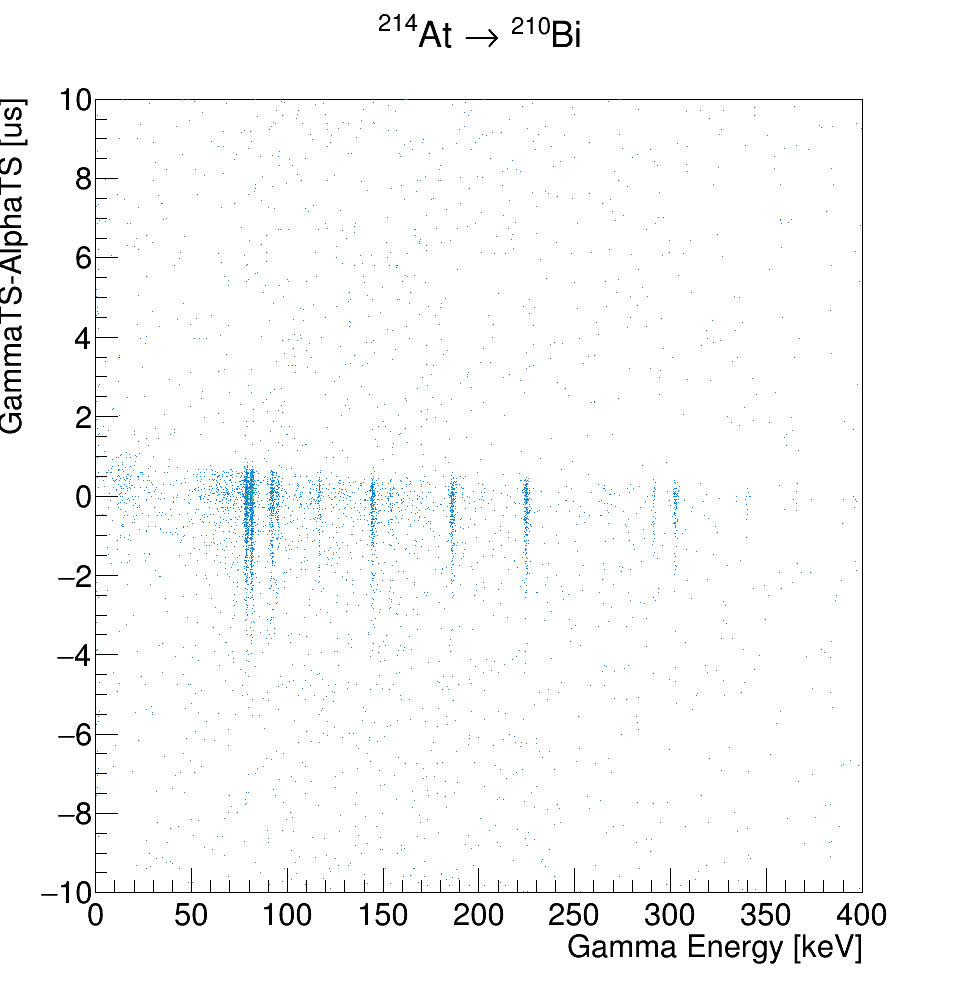
\includegraphics[width=\textwidth]{GTvsG_214At.png}
			\end{overlayarea}
		\end{column}
	\end{columns}	
\end{frame}

\begin{frame}{Mass 226}	
	\centering
	\vspace{-0.05\textheight}
	\only<1>{\hspace*{-0.05\textwidth}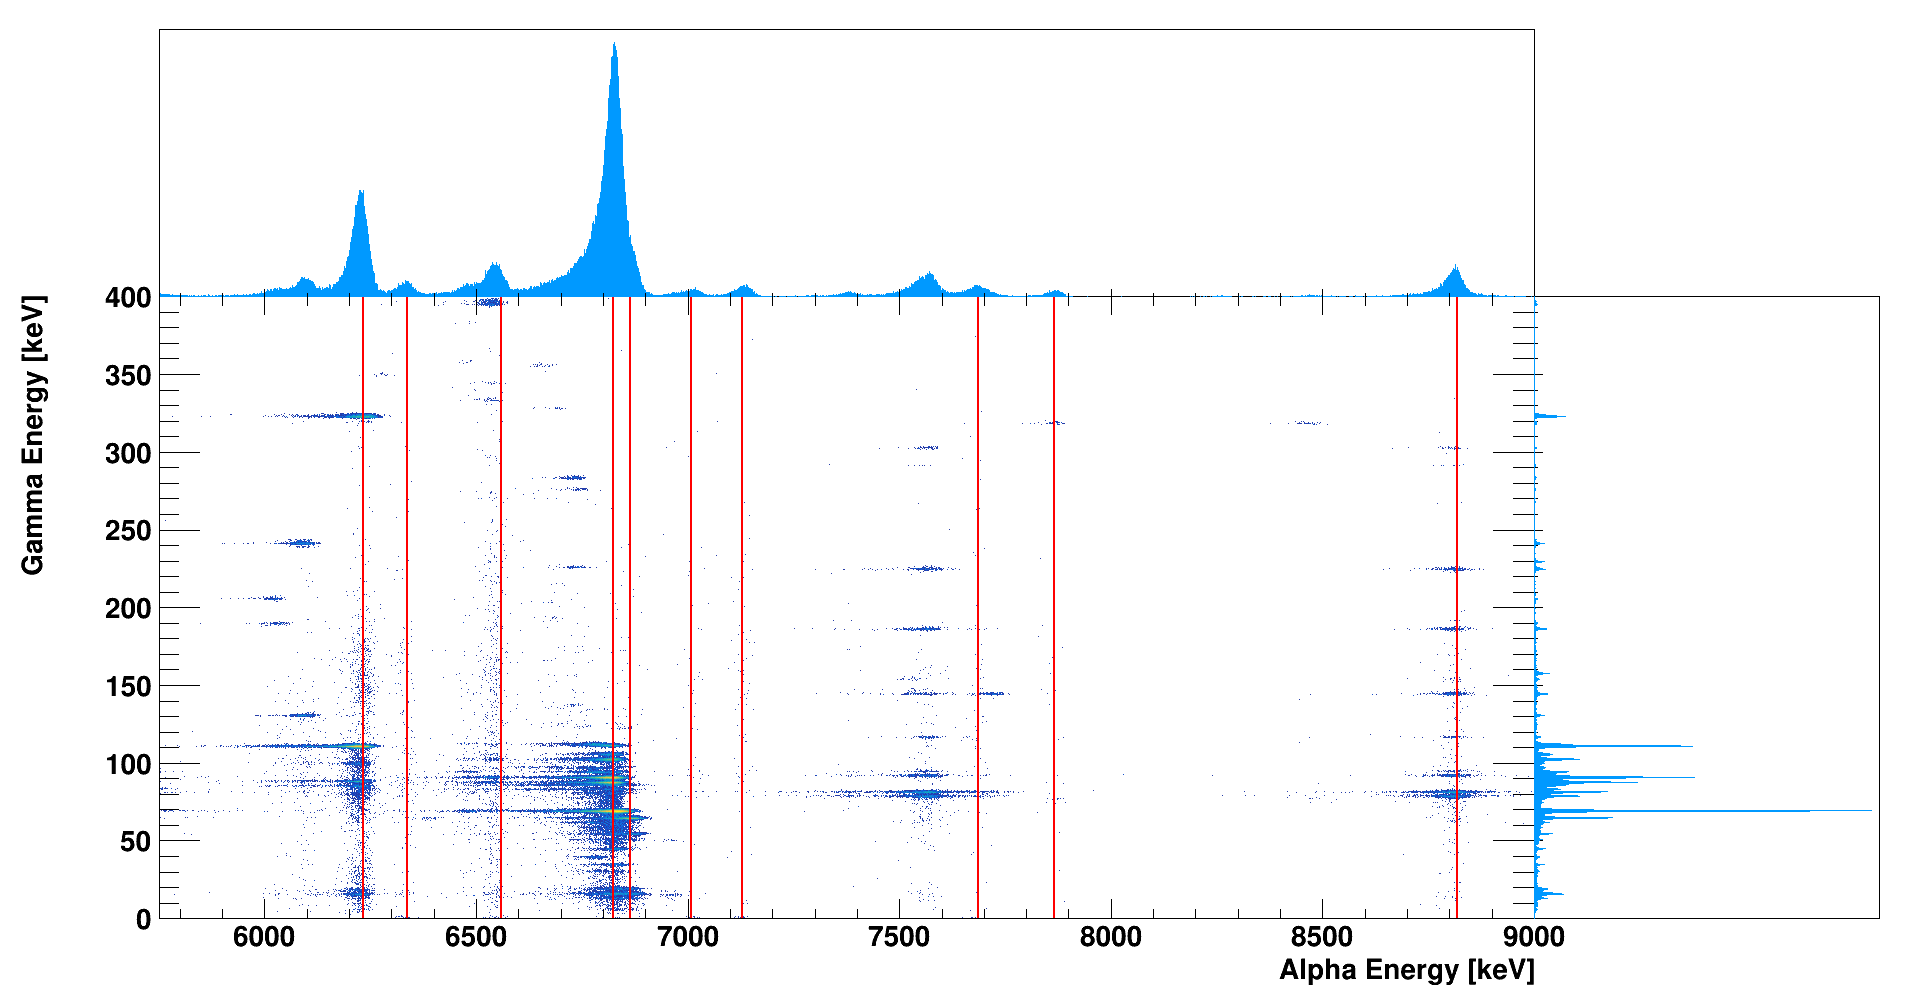
\includegraphics[width=1.1\textwidth]{AvsG_2us.png}}%
	\only<2>{\hspace*{-0.05\textwidth}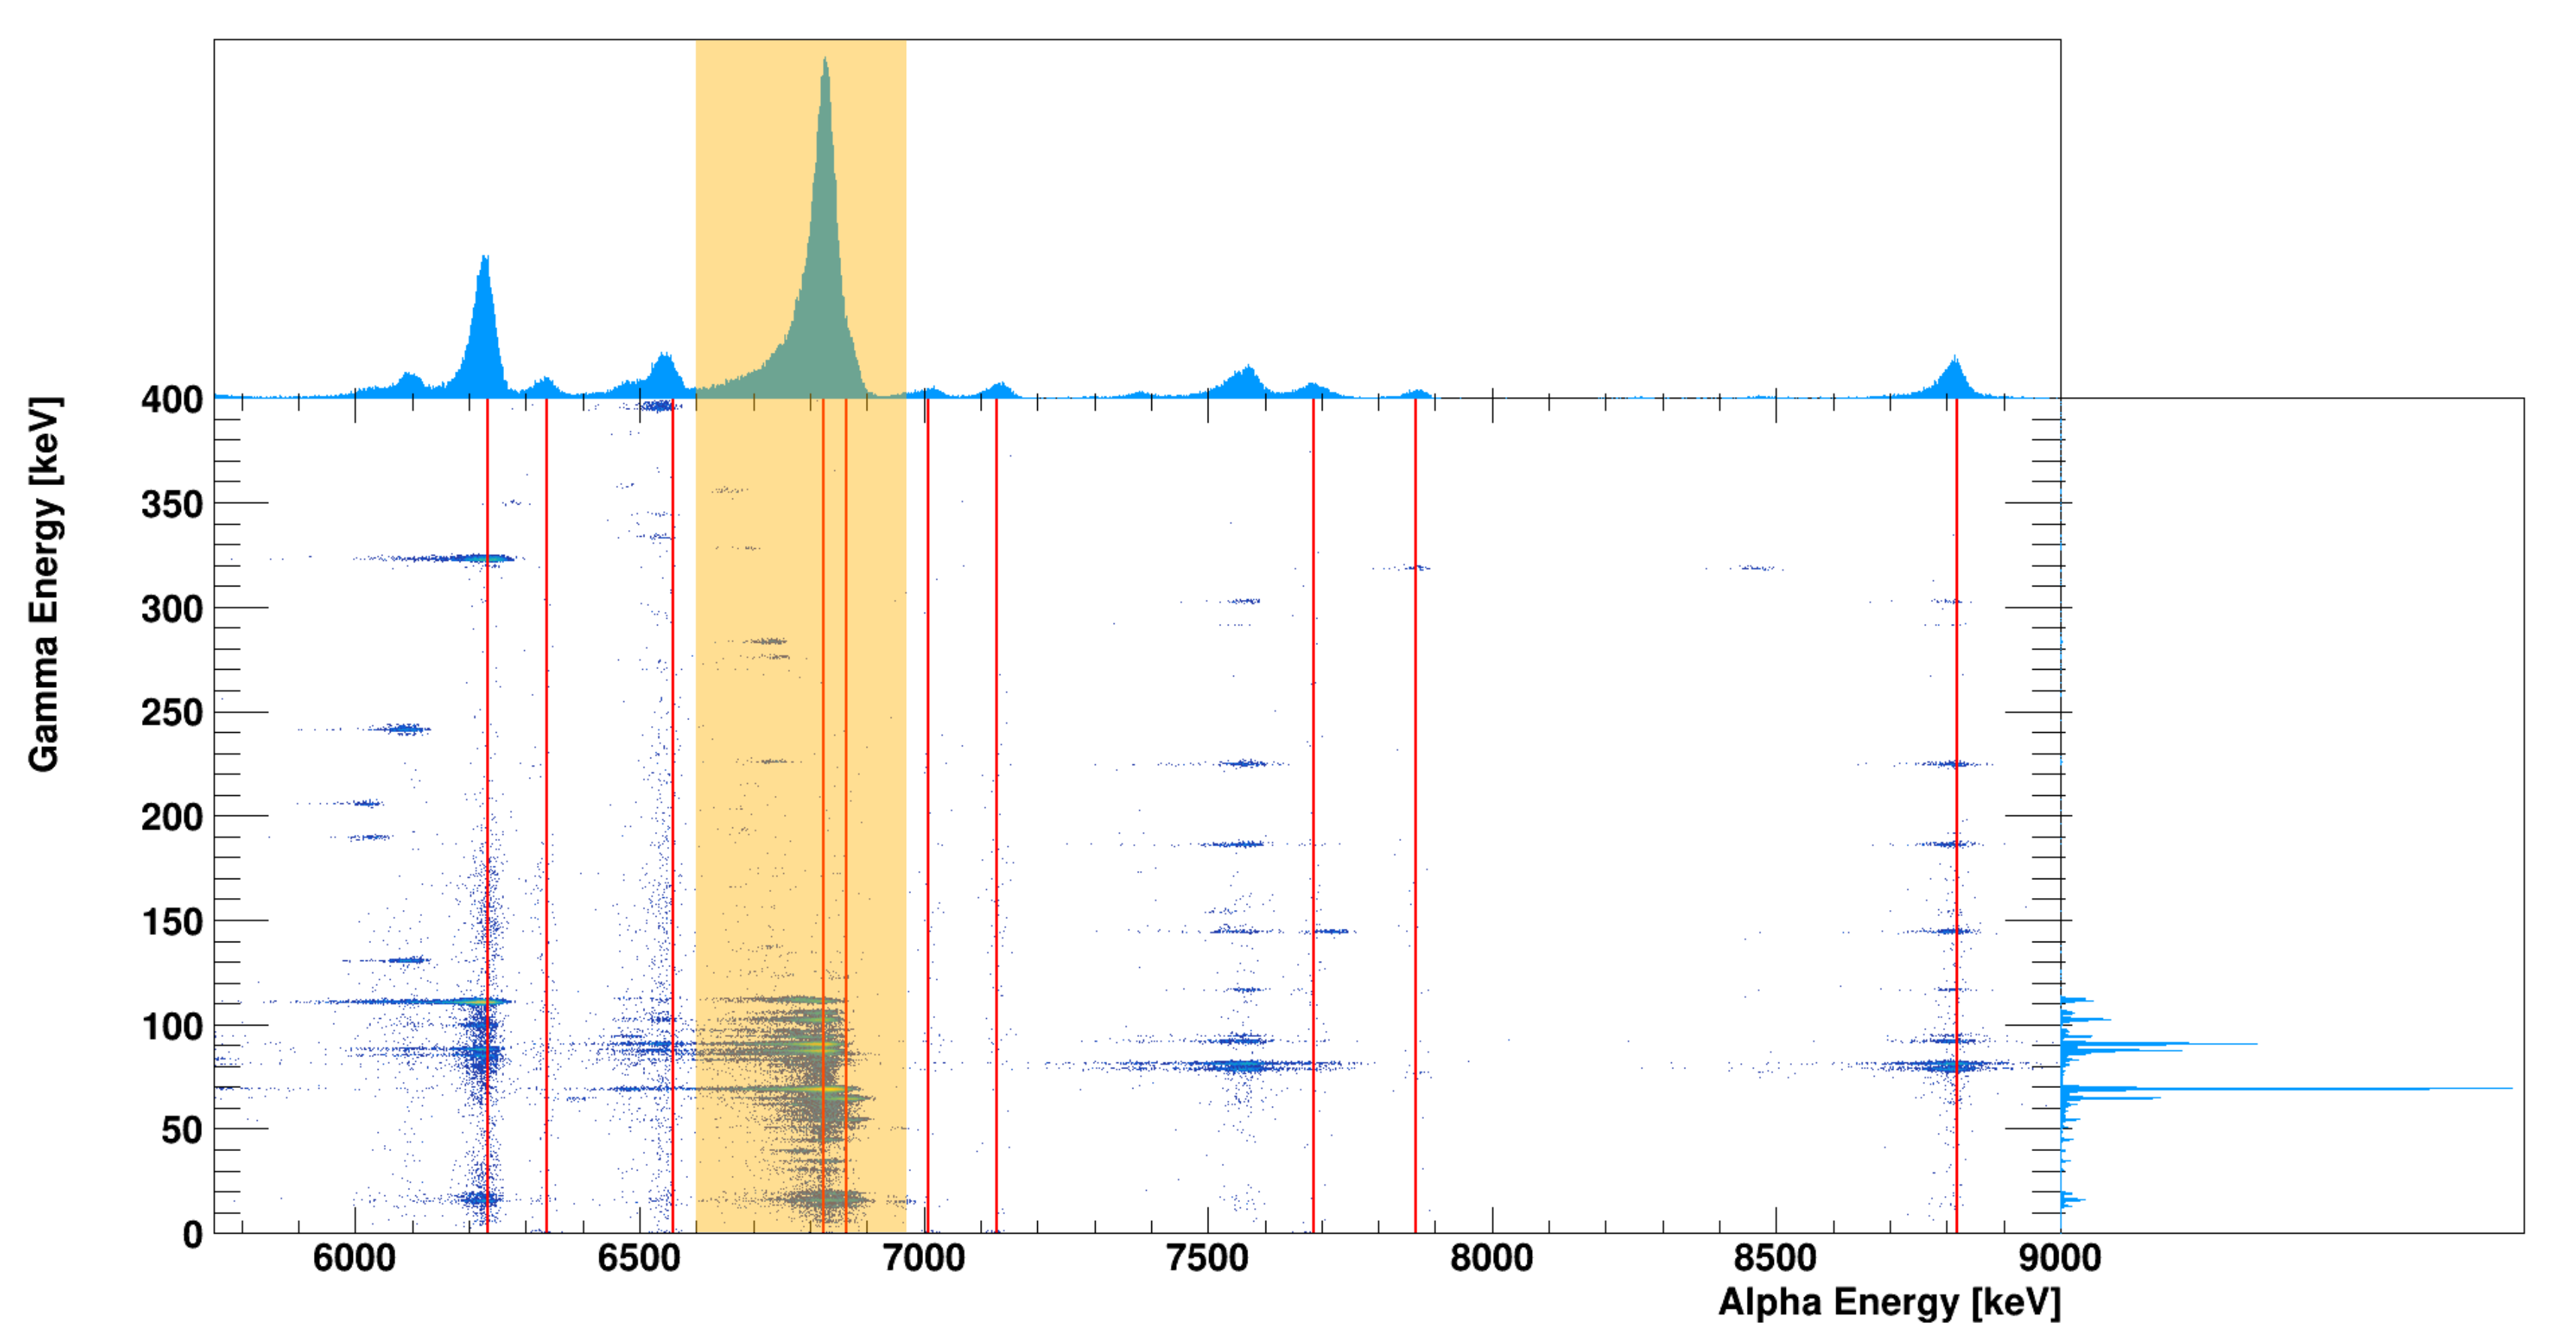
\includegraphics[width=1.1\textwidth]{AvsG_2us_226PaGate.png}}%
\end{frame}

\begin{frame}{$^{226}$Pa Gamma spectrum}	
	\centering
	\vspace{-0.05\textheight}
	\only<1>{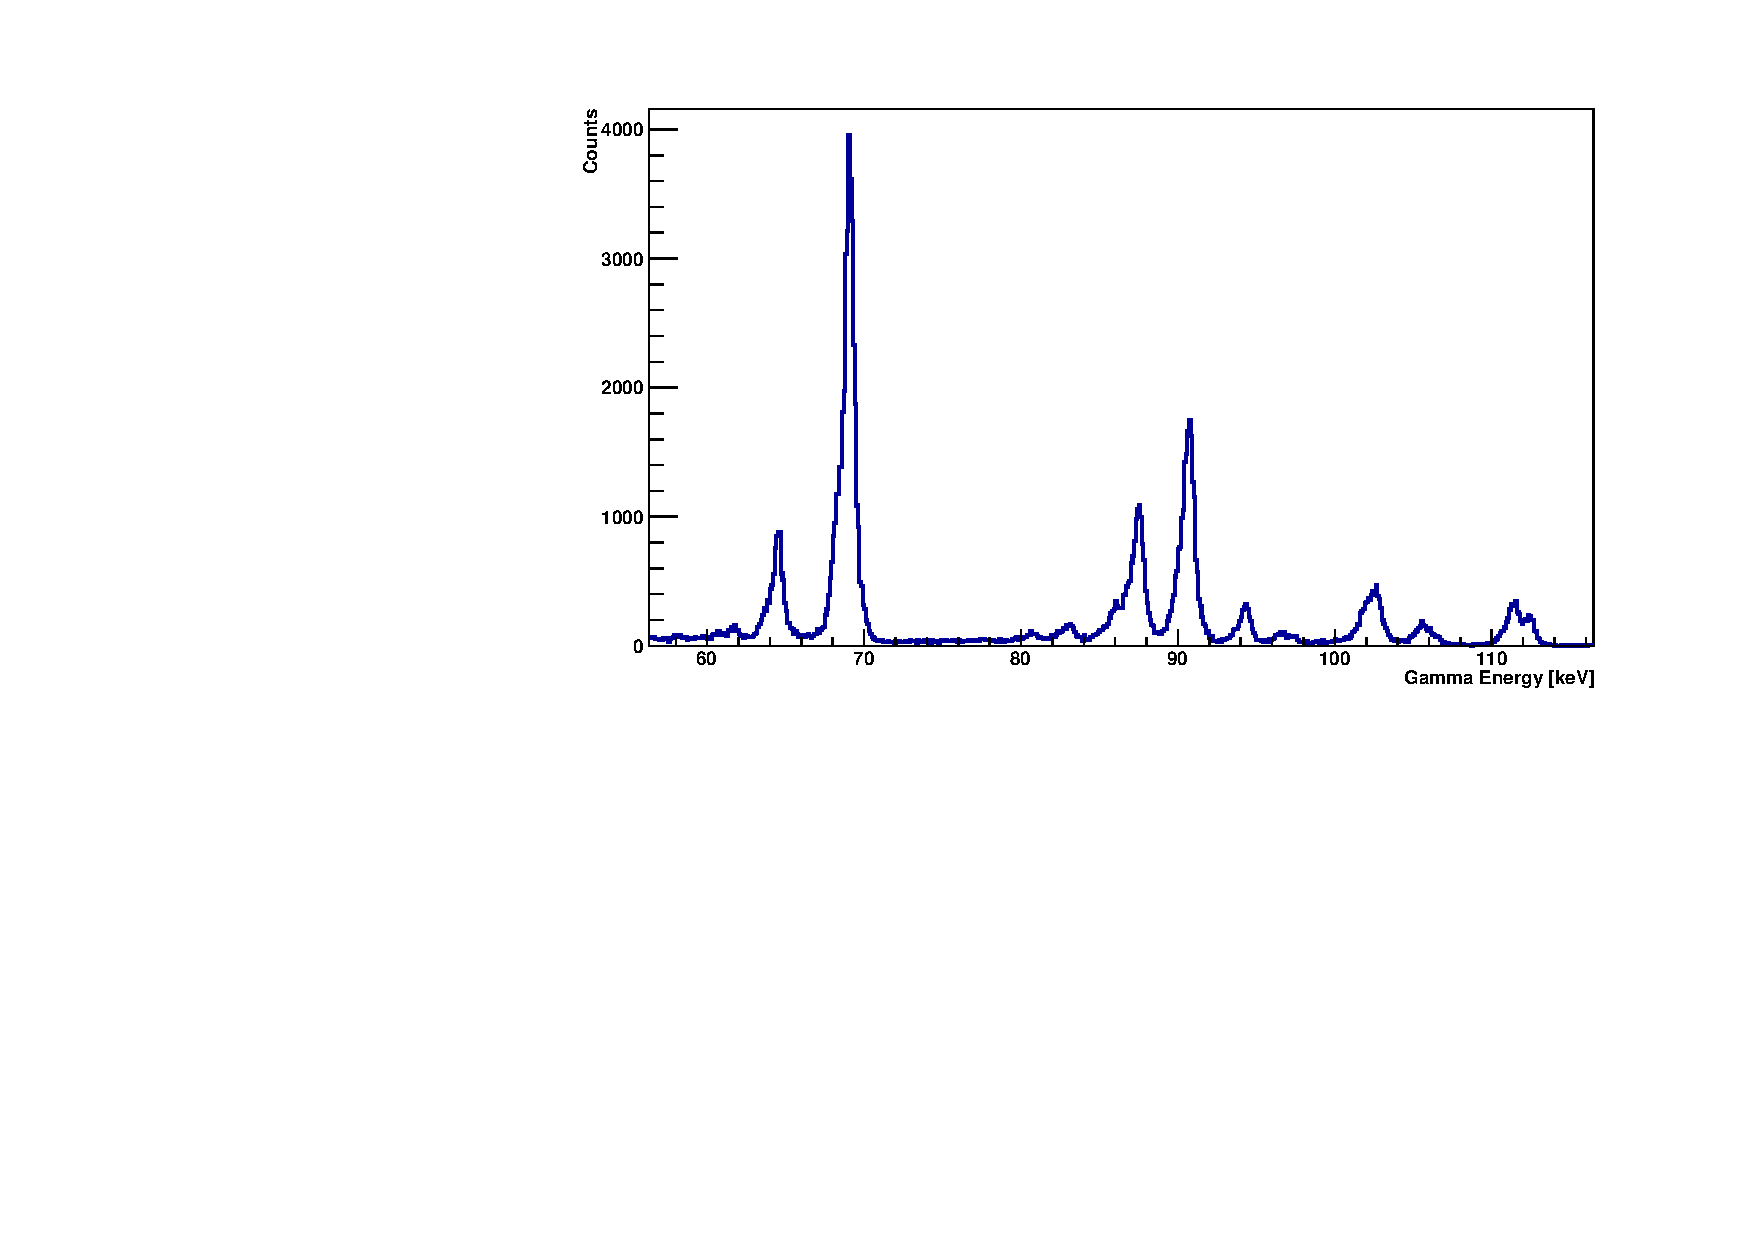
\includegraphics[width=1\textwidth]{GSpectra_226Pa_badCal.pdf}}%
	\only<2>{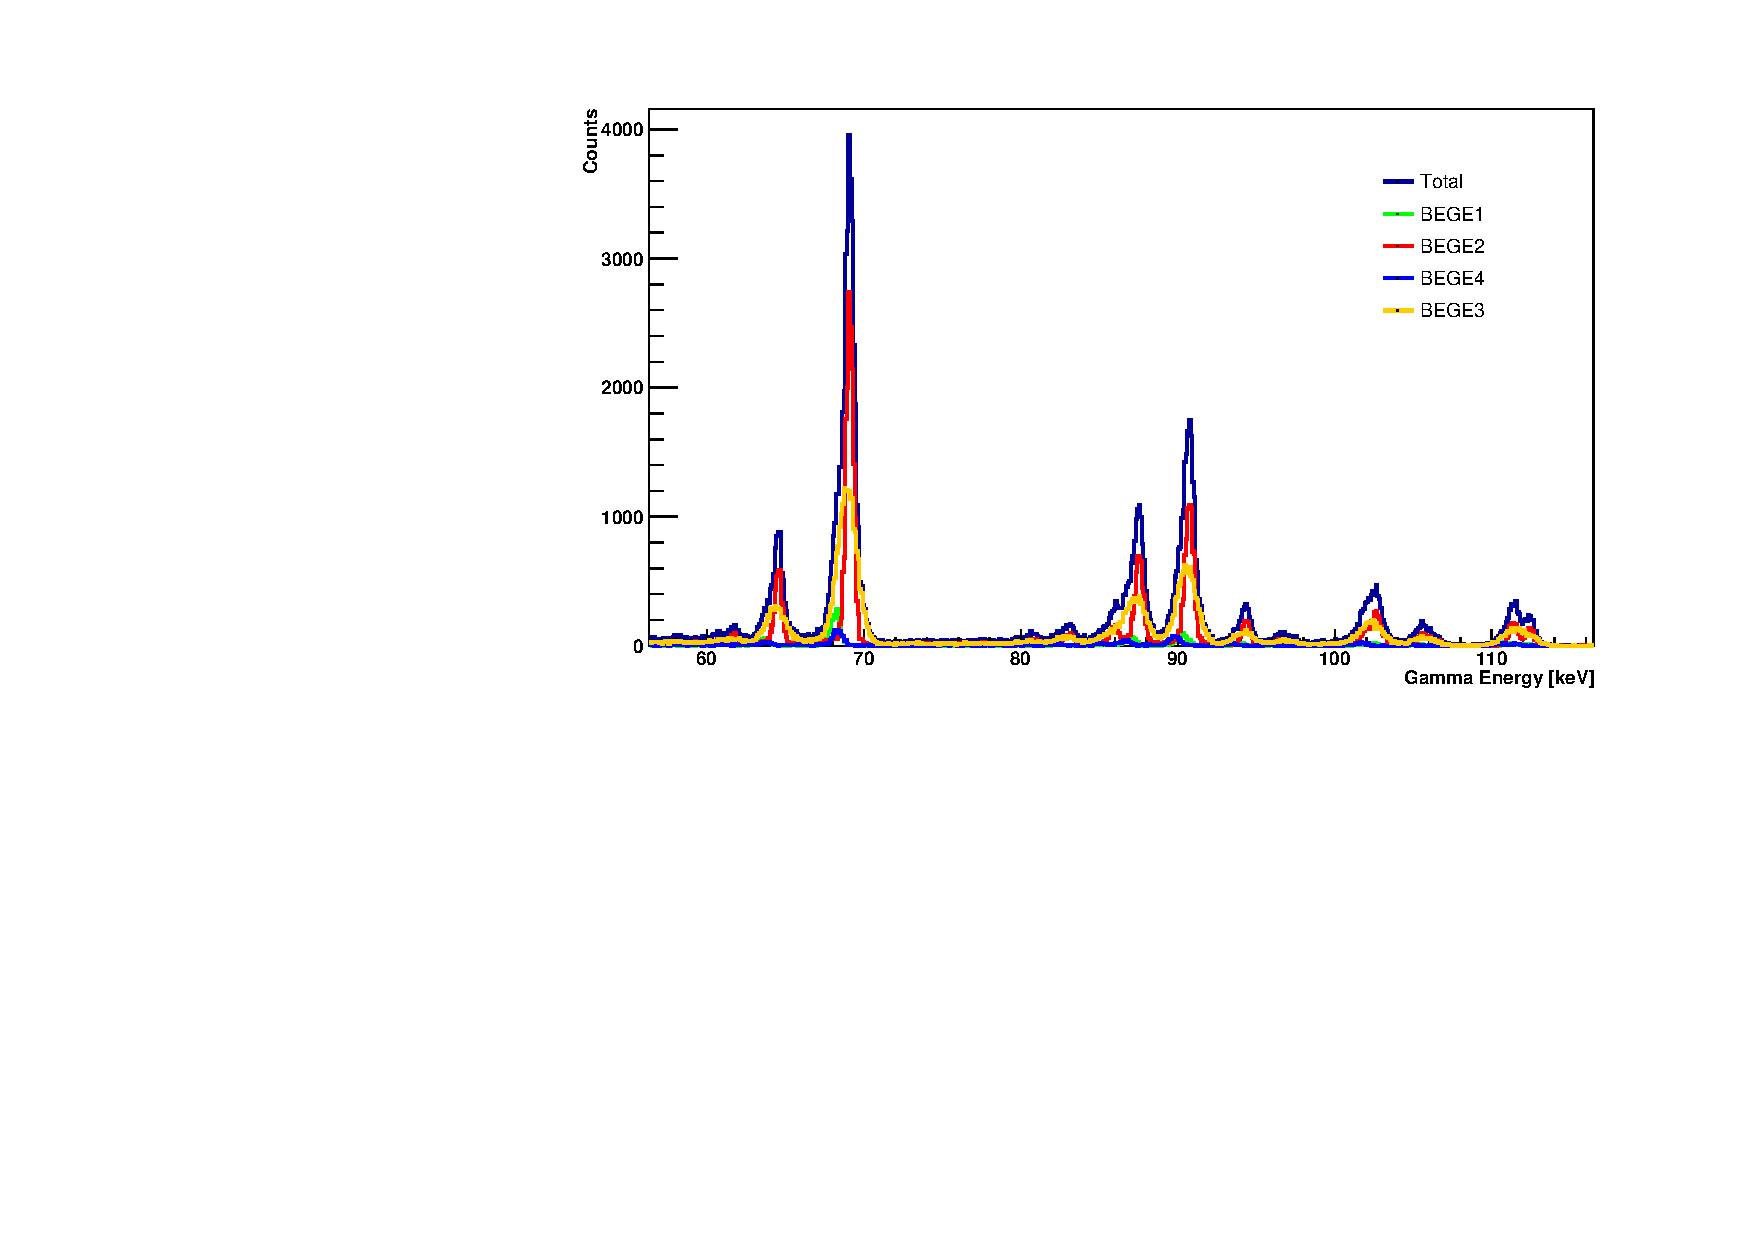
\includegraphics[width=1\textwidth]{GSpectra_226Pa_badCal_singleBEGE.pdf}}%
\end{frame}

\begin{frame}{$^{226}$Th Gamma spectrum}	
	\centering
	\vspace{-0.05\textheight}
	\only<1>{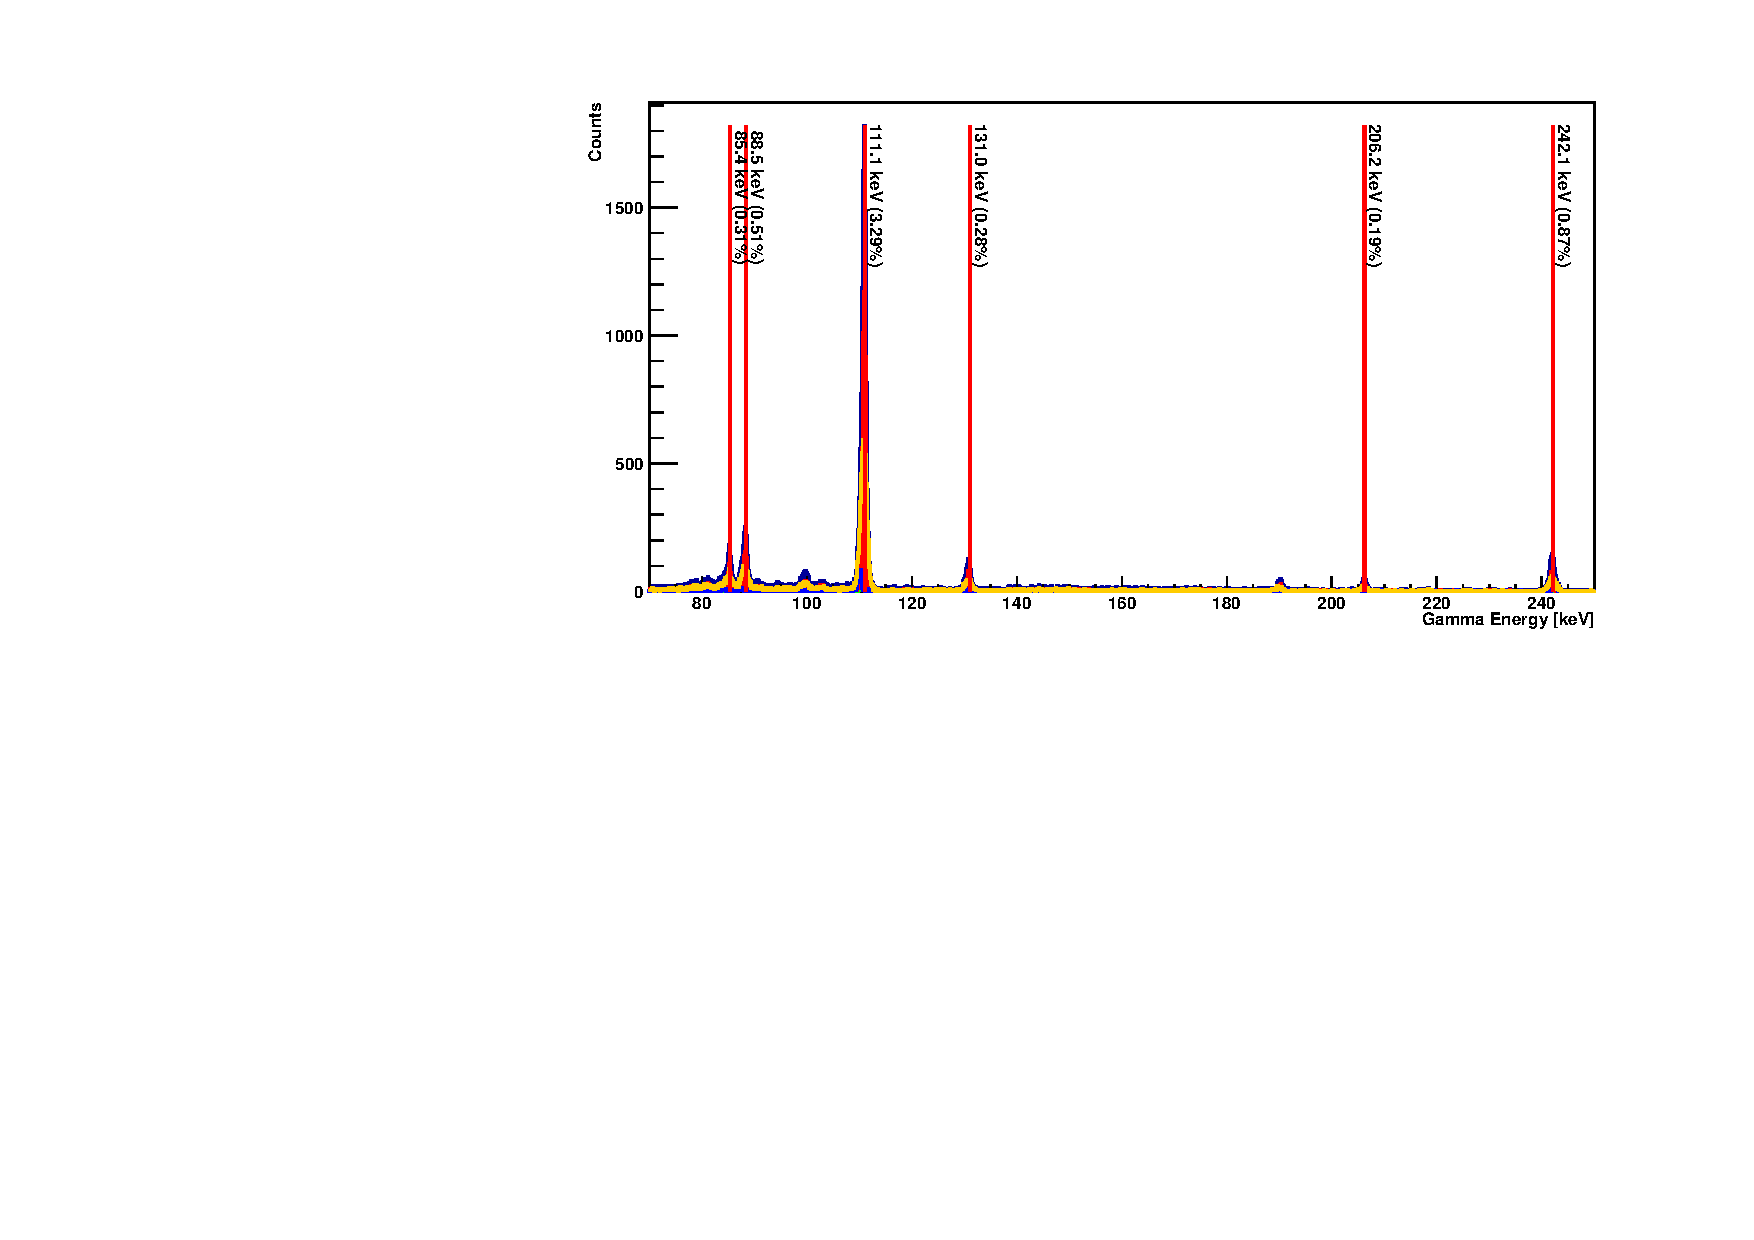
\includegraphics[width=\textwidth]{GSpectra_226Th_badCal_singleBEGE.pdf}}%
\end{frame}

\begin{frame}{$^{226}$Pa Gamma spectrum}
	\begin{columns}
		\begin{column}{0.5\textwidth}
			\begin{overlayarea}{\textwidth}{0.5\textheight}
				\centering
				\vspace{-0.1\textheight}
				Before\\
				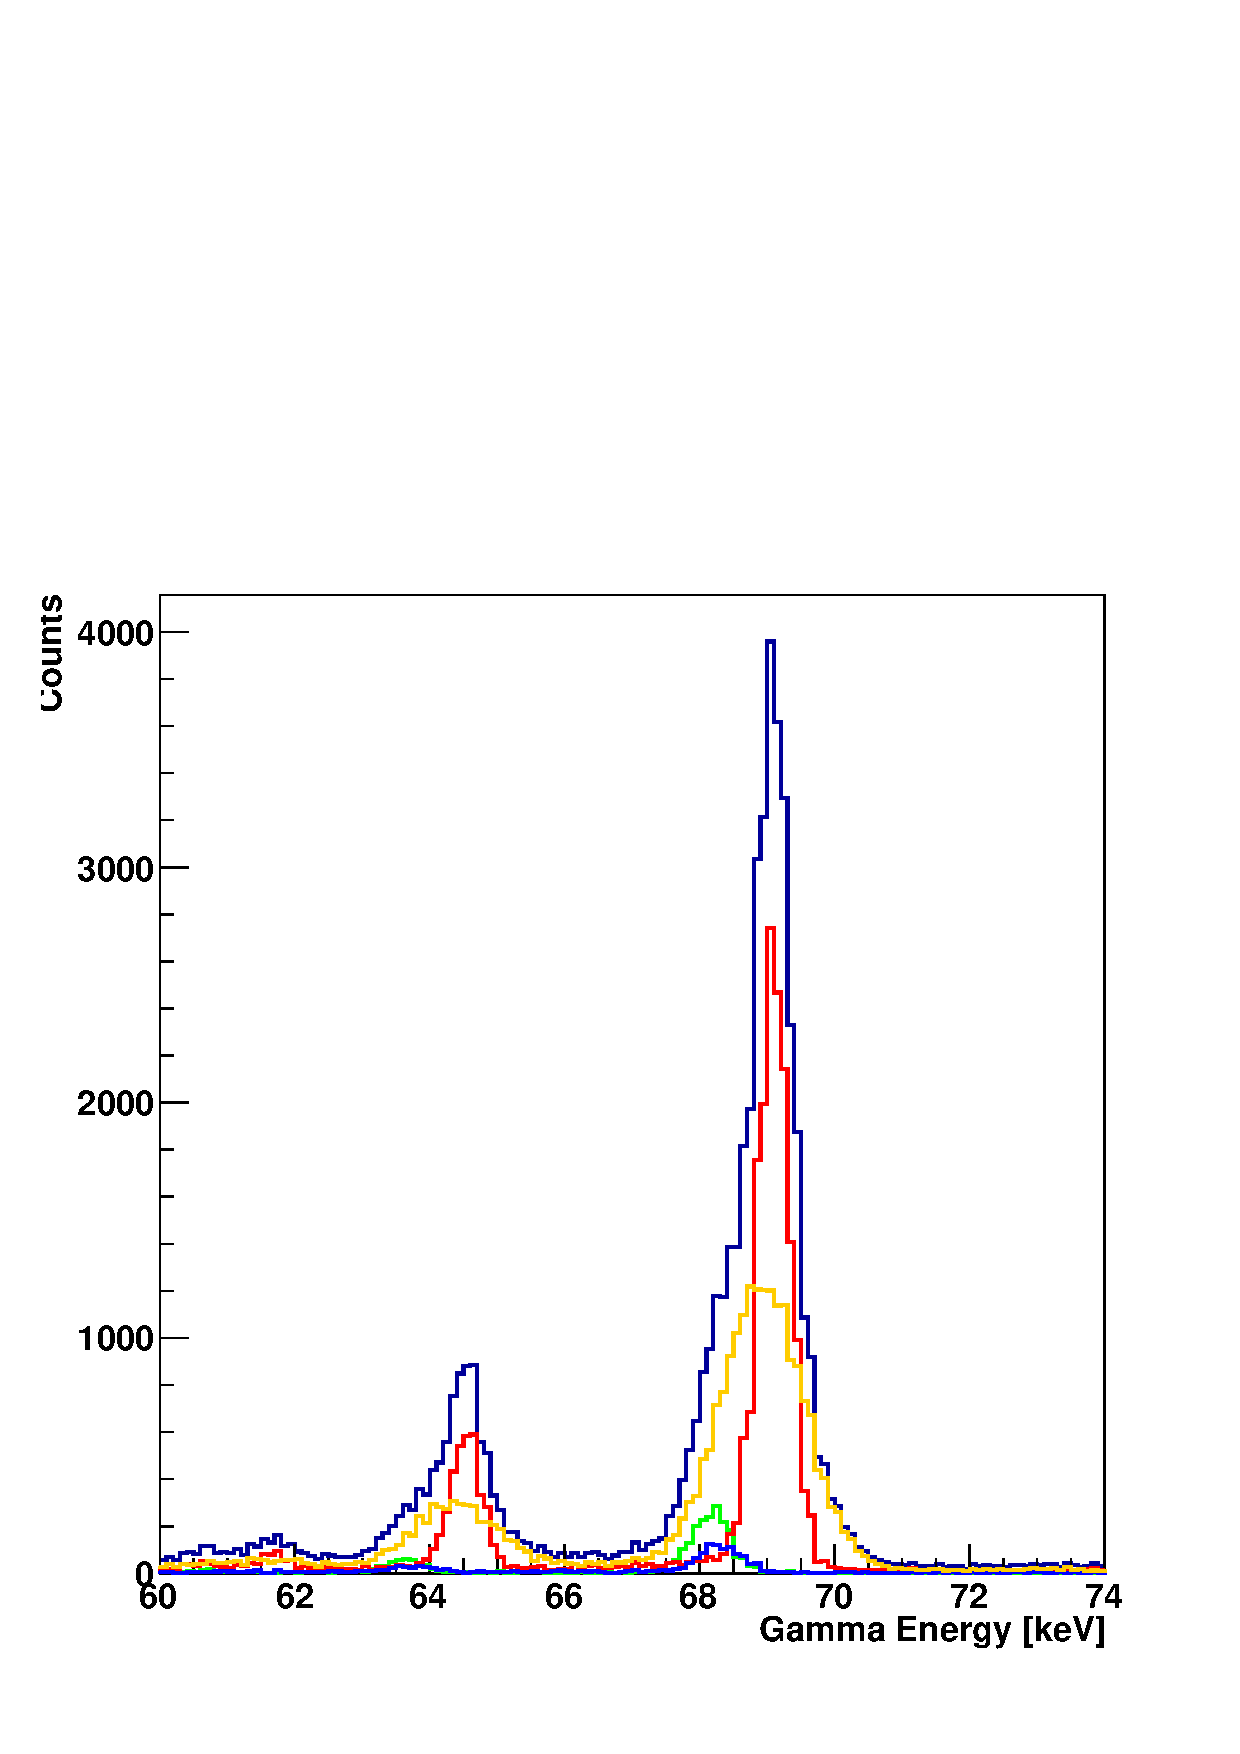
\includegraphics[width=\textwidth]{GSpectra_226Pa_badCal_zoom.pdf}
			\end{overlayarea}
		\end{column}
		\begin{column}{0.5\textwidth}
			\begin{overlayarea}{\textwidth}{0.5\textheight}
				\centering
				\vspace{-0.1\textheight}
				After\\
				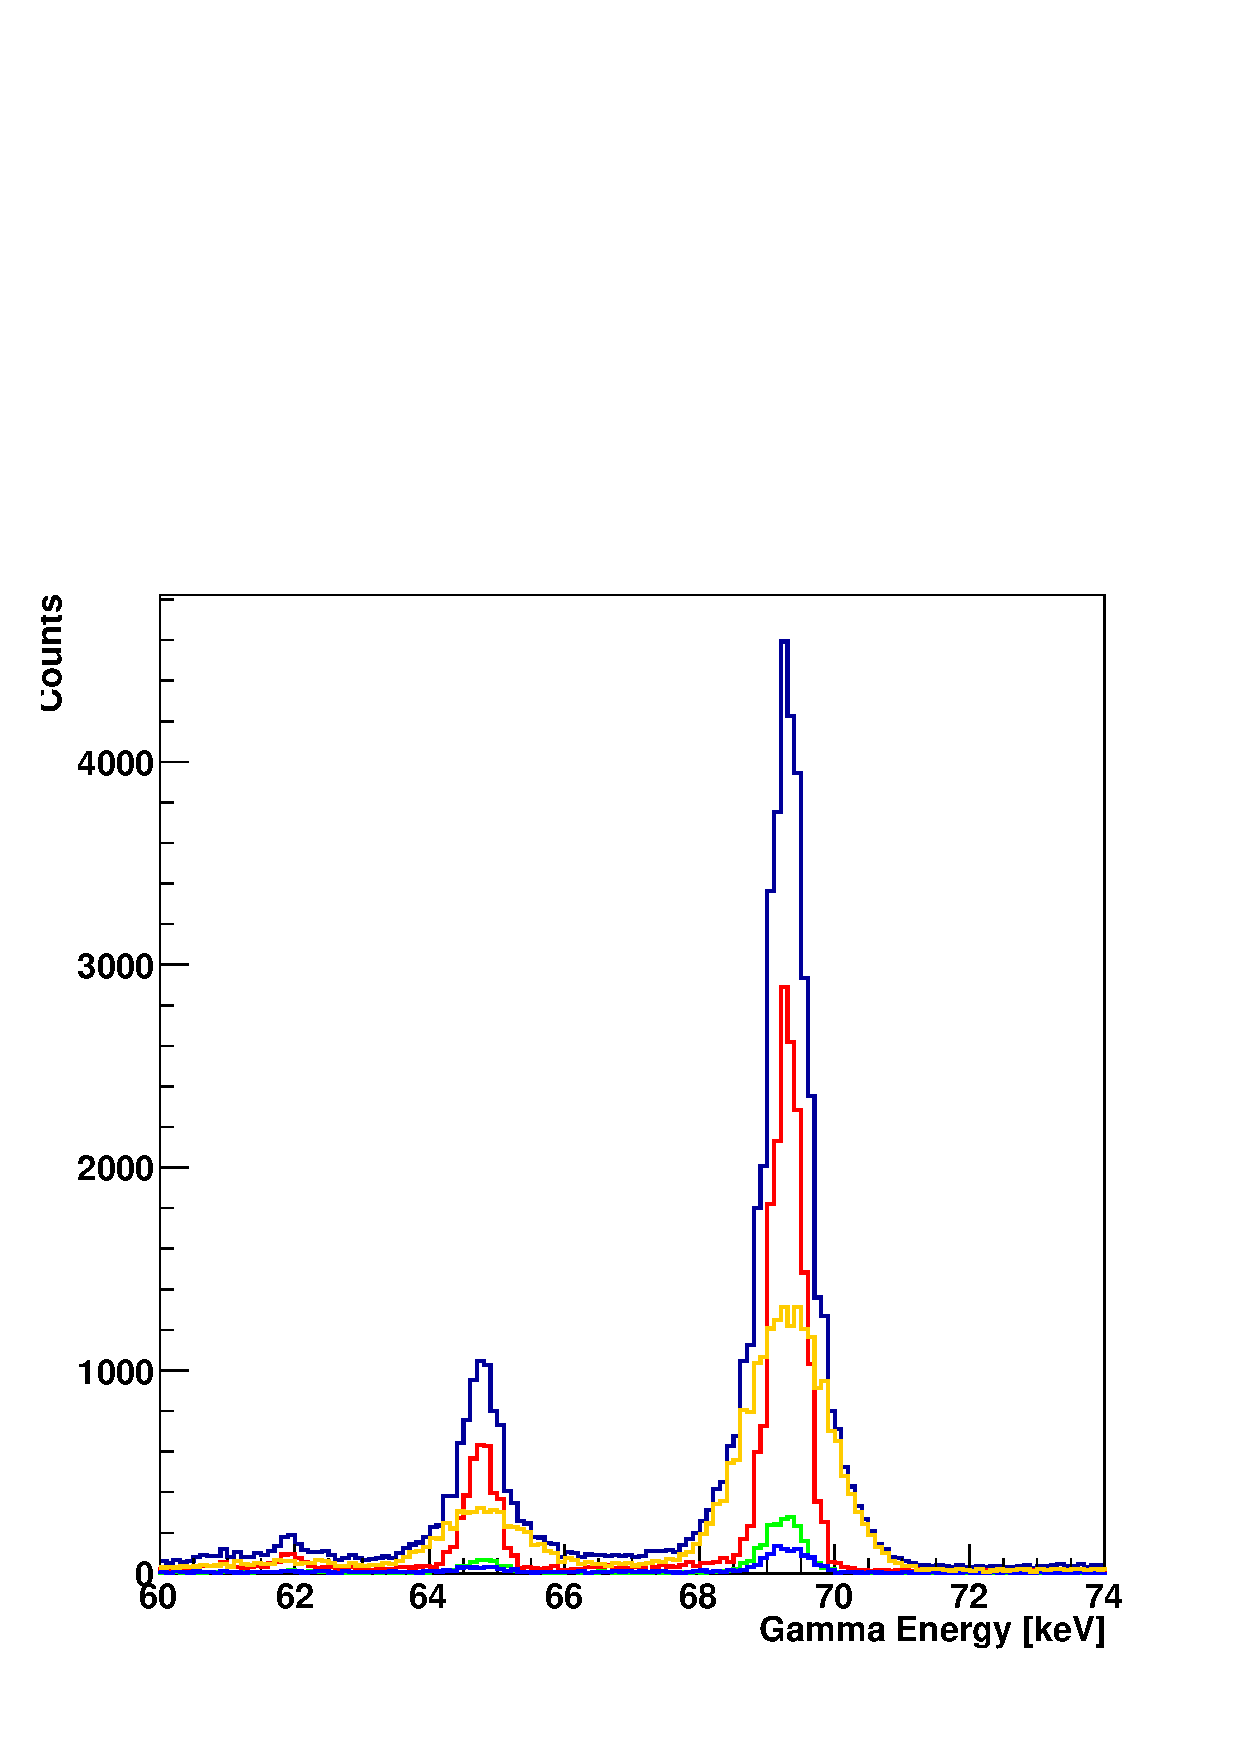
\includegraphics[width=\textwidth]{GSpectra_226Pa_zoom.pdf}
			\end{overlayarea}
		\end{column}
	\end{columns}	
\end{frame}

\begin{frame}{$^{226}$Pa $\alpha\gamma$ coincidence}	
	\centering
	\vspace{-0.05\textheight}
	\hspace*{-0.05\textwidth}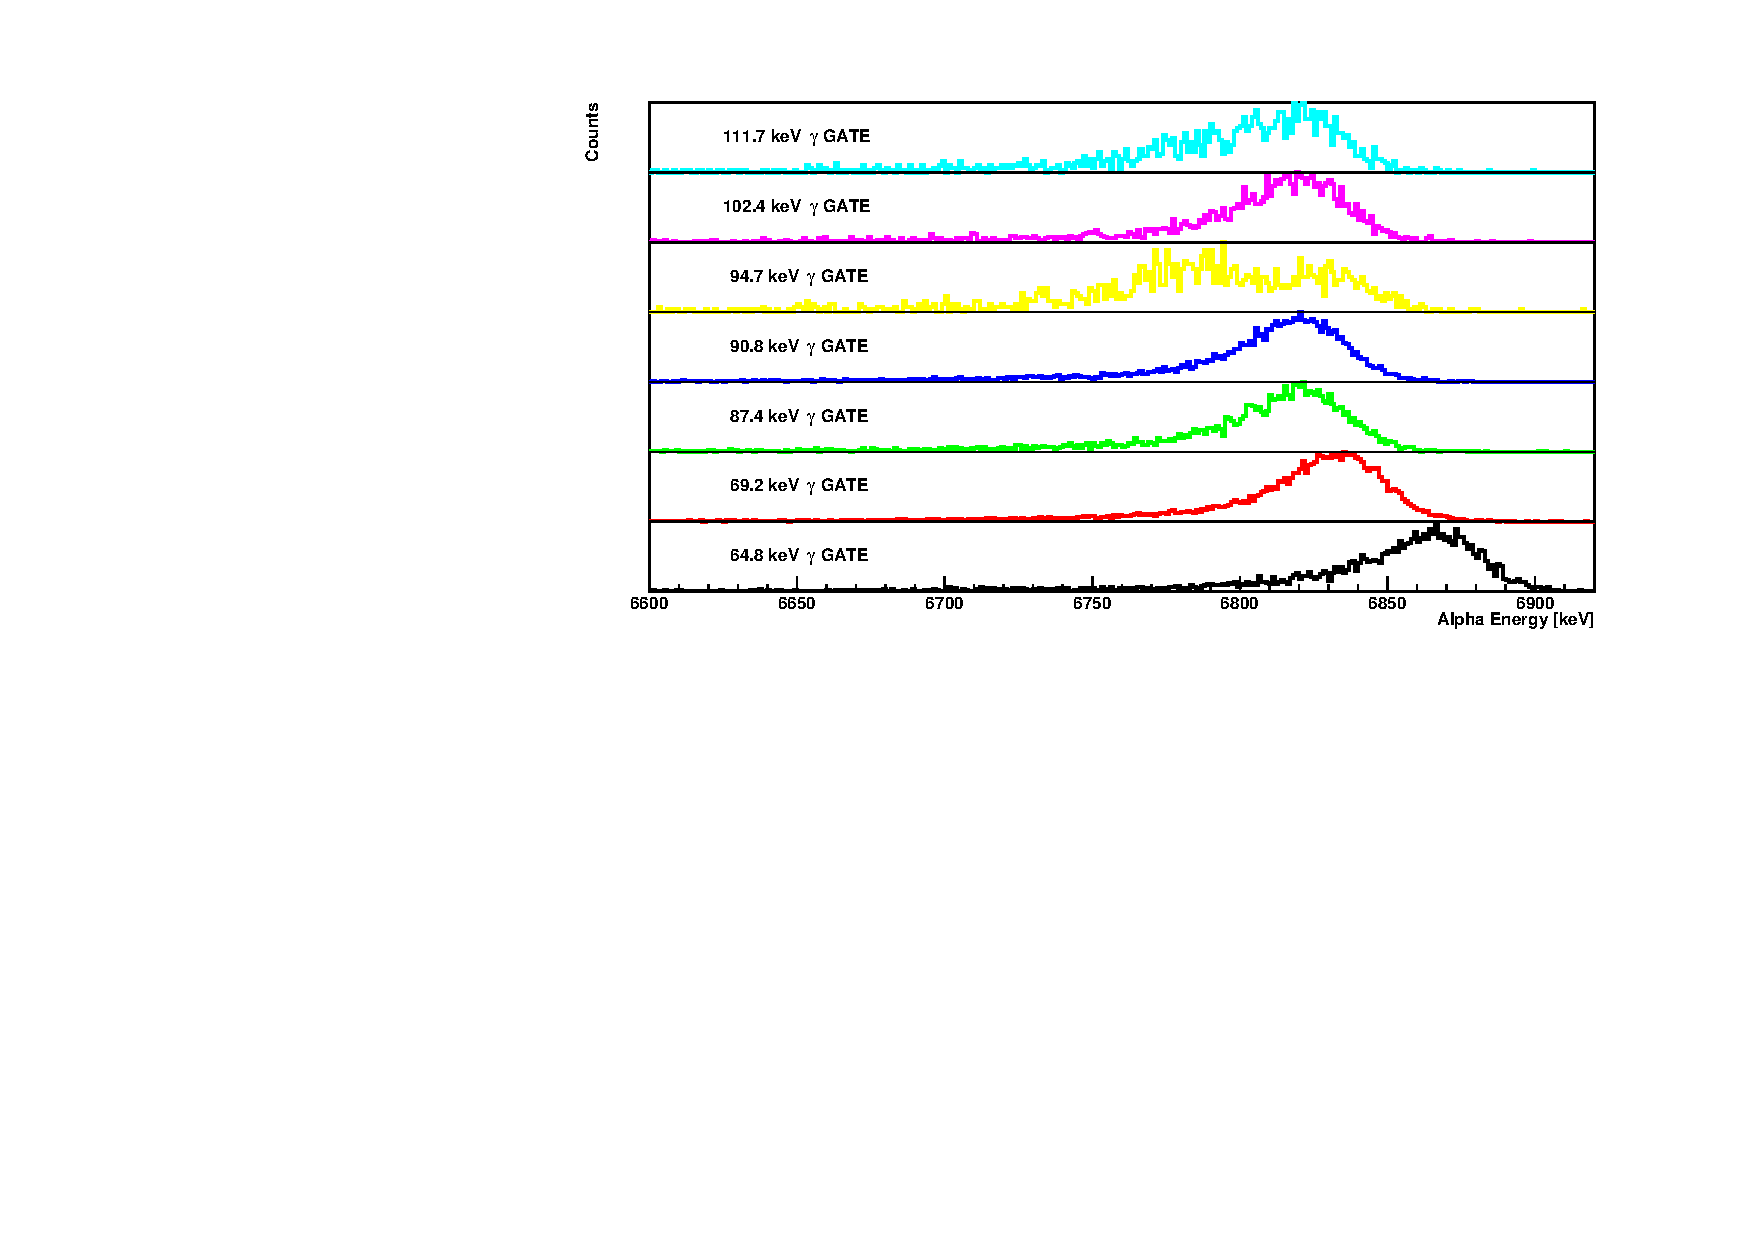
\includegraphics[width=1.1\textwidth]{ASpectra_226Pa_GammaGated.pdf}%
\end{frame}


\begin{frame}{$^{226}$Th electrons?}	
	\centering
	\vspace{-0.05\textheight}
	\hspace*{-0.05\textwidth}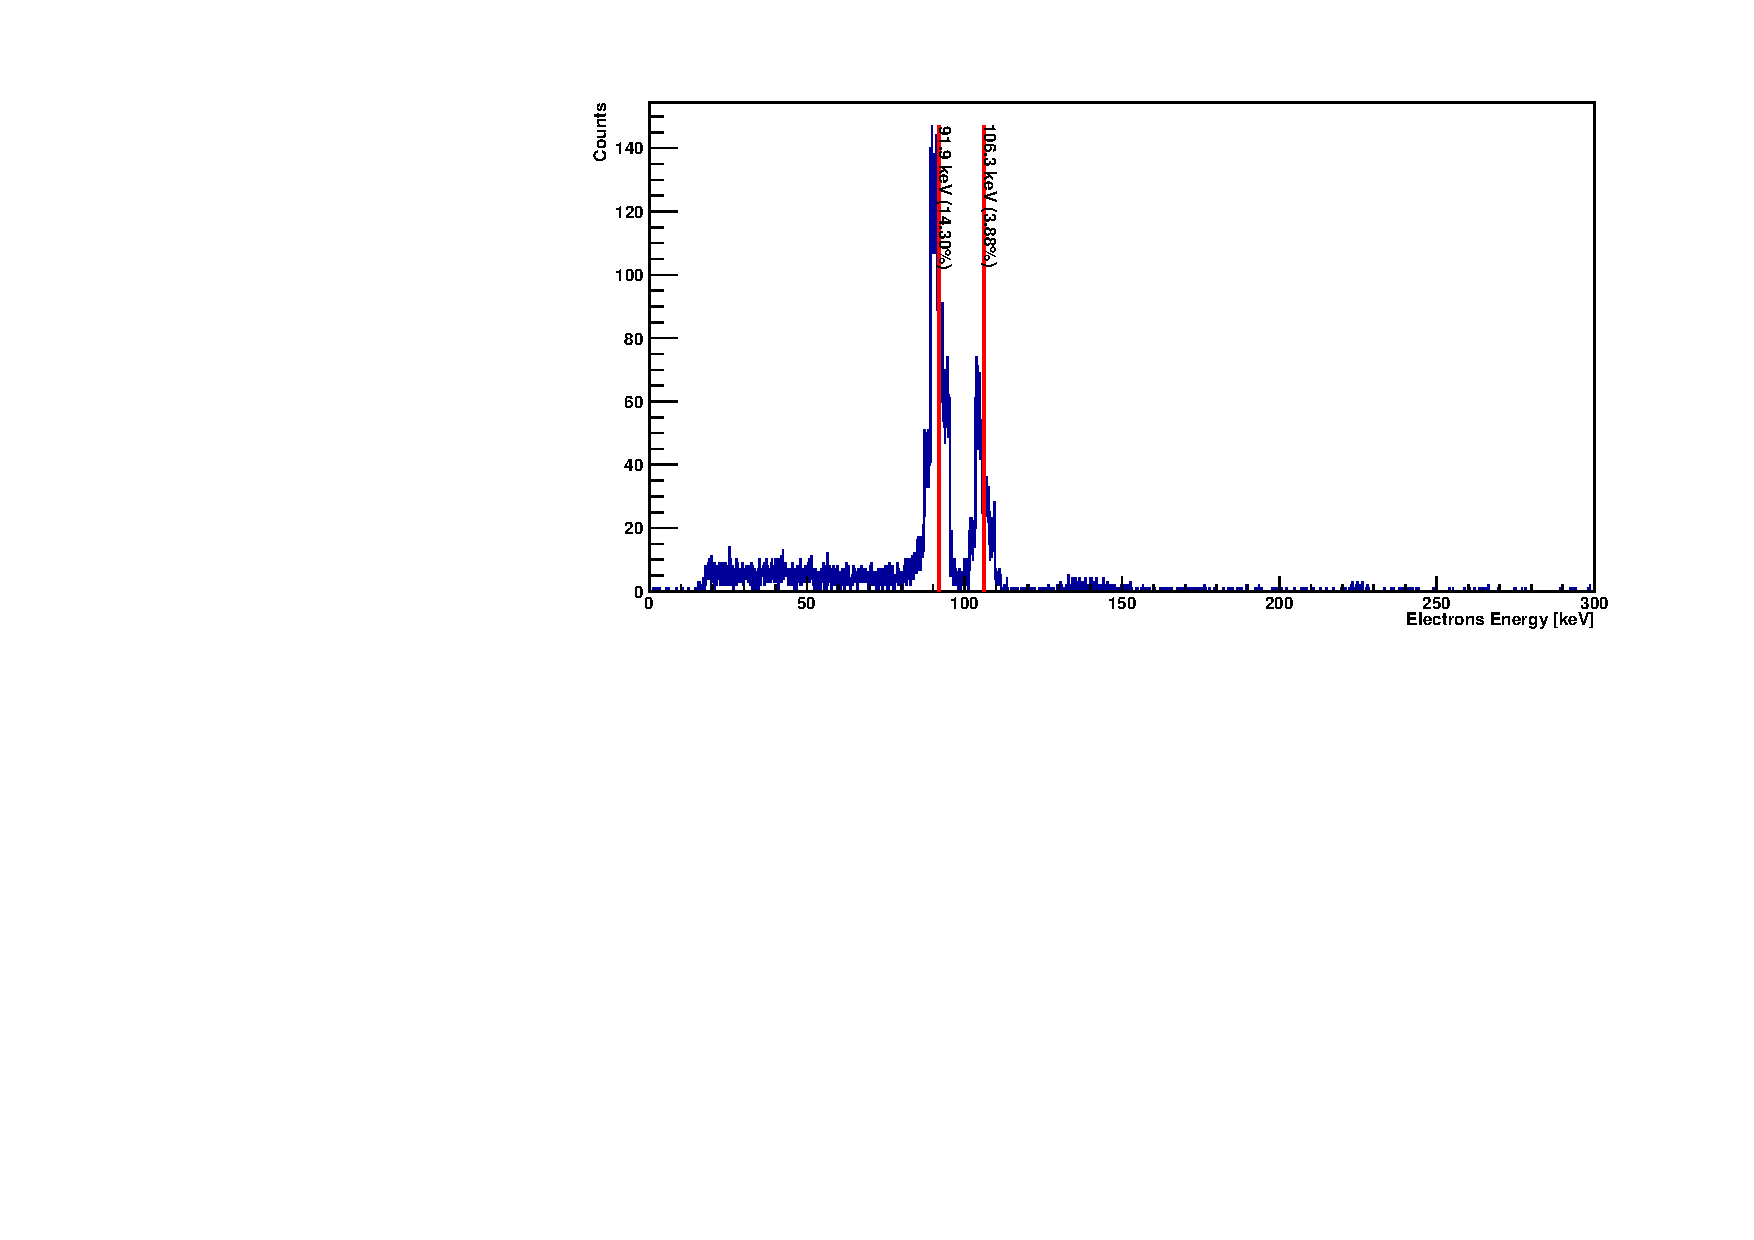
\includegraphics[width=1.1\textwidth]{ESpectra_226Th.pdf}
\end{frame}


\end{document}